%!TEX root = ../dissertation.tex
\begin{savequote}[75mm]
	Negative advertising is the crack cocaine of politics.
	\qauthor{Senator Tom Daschle}
\end{savequote}

\chapter{La campagna politica negativa}
\label{chap:negative}

Negli ultimi tre decenni le scienze sociali hanno indagato a fondo i messaggi politici negativi. I candidati investono molto nelle strategie delle loro campagne che rappresentano la modalità principale di comunicazione con gli elettori, dagli stikers, volantini, cartelloni elettorali, alle interviste e spots sui media tradizionali, fino alle campagne online tramite contenuti sponsorizzati sulla propria pagina e quella del partito sui vari social networks.

Questi messaggi elettorali possono avere un'accezione prevalentemente positiva, cioè volta a diffondere le proprie proposte e i propri punti di forza, oppure possono avere un'accezione più negativa quando si cerca di far risaltare le debolezze dell'avversario, criticandolo o contrapponendosi al suo programma politico. Su questa distinzione si genera la definizione di “campagna politica negativa”.

\section{La definizione}
Come riportato da Walter \citep{walter2014}, delineare il \textit{negative campaign} può risultare difficile. Diverse sono le definizioni in uso all'interno della  comunità accademica. Nel libro di Swint \citep{swint1998} vengono discusse molte di queste possibili interpretazioni, considerando che, a livello di opinione pubblica, molt* faticano a convergere su un solo  significato , generando, così,  fraintendimenti. A riguardo viene citato uno studio di Surlin e Gordon del 1977 \citep{surlin1977} in cui si mostra come la maggior parte degli elettori veda le campagne negative come quelle in cui è contenuto un attacco scorretto nei confronti di un avversario. In questi casi si sottintende una definizione valutativa che fa riferimento alla illegittimità degli attacchi. Si tratta, però, di una definizione difficilmente quantificabile, che lascia molto spazio all'interpretazione soggettiva. Secondo questo approccio, le campagne negative vengono anche chiamate "dirty" oppure "poison politics". Jamieson \citep{jamieson1993} cita vari esempi in cui gli attacchi risultano palesemente falsi come quello in cui Bush ha attaccato il rivale Dukakis dicendo che era "praticamente contro ogni arma che abbiamo sviluppato". Tale affermazione ha spinto Dukakis a girare uno spot in cui guidava un carro armato M1, per togliere ogni dubbio agli elettori, risultando però ancora più debole, poiché costretto sulla difensiva, e punito in seguito dagli elettori alle urne. Con esempi come questo l'autore vuole far capire come la "dirty politics" possa risultare efficace se utilizzata intelligentemente, nonostante si possa basare anche sulla palese menzogna, strumento che dovrebbe essere responsabilmente evitato da candidati alle elezioni.
\begin{wrapfigure}{r}{7cm}
	\centering
	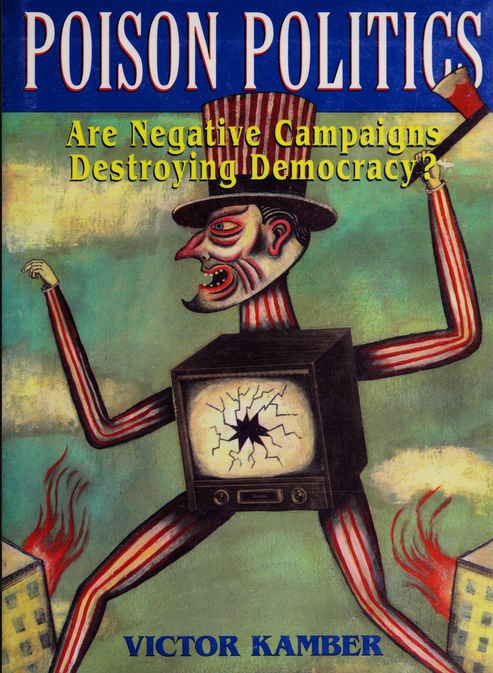
\includegraphics[width=5.5cm]{figures/poison}
	\caption{Copertina del libro di Kamber: "Poison politics: Are negative campaigns destroying democracy?", 1997}
	\label{poison3}
\end{wrapfigure}

Anche Kamber \citep{kamber1997}, come viene chiaramente trasmesso dalla copertina del suo libro [Fig.~\ref{poison3}], si interroga su come la \textit{poison politics} possa avere conseguenze sulla sorti della democrazia. In questo filone di discorso il \textit{negative campaign} risulta interpretato nella sua definizione valutativa, con l’obiettivo di tracciare dei confini che il discorso politico non dovrebbe oltrepassare per evitare che possa avere conseguenze sulla pacifica convivenza.
Nel libro di Kamber viene descritta la responsabilità necessaria per candidarsi a una carica pubblica, rimarcando quanto sia importante per tutta la comunità che i rappresentanti politici evitino scorrettezze in campagna elettorale, come l'utilizzo di menzogna, calunnia e attacchi a caratteristiche personali non influenti ai fini della candidatura. L'autore, noto senatore democratico statunitense e consulente per campagne elettorali dei rappresentati di questo schieramento, quindi molto focalizzato nell'attacco di parte dei "evil Republicans",  arriva a descrivere queste tattiche come "anti-politica" per gli effetti nefasti che possono avere sulla fiducia degli elettori nelle istituzioni in generale.

La definizione di \textit{negative campaign} largamente più utilizzata in letteratura, soprattutto negli studi quantitativi come il nostro, risulta però essere quella direzionale che vi fa rientrare tutti i tipi di attacchi al di là della valutazione di merito, includendo anche le critiche del tutto legittime, argomentate senza insulti o toni eccessivi e necessarie al processo democratico. In base a questo approccio la campagna positiva risulta per antitesi quella in cui si propone in modo costruttivo la propria posizione e le proprie proposte senza alcun riferimento a quelle degli avversari.

Da alcuni autori \citep{jamieson1997} \citep{jamieson1998}, è stata proposta una definizione direzionale tripartita che tiene conto anche delle campagne comparative come separate da quelle negative e positive. In particolare è stata proposta la divisione in "advocacy" con argomenti in favore del candidato, "attacks" con riferimenti agli avversari e "comparison" che unirebbe entrambi i primi due tipi di campagna. Questa definizione viene applicata allo studio dei singoli spot pubblicitari dei politici statunitensi durante le elezioni del '96. In questa campagna vengono riscontrate differenze molto significative tra i due politici presi in considerazione riguardo in particolare alle campagne comparative, dimostrando come questa categoria non risulti superflua, ma invece importante per discernere al meglio i messaggi elettorali negativi che citano l'avversario senza citare la propria posizione.

Lau e Pomper \citep{lau2004} criticano questa ulteriore suddivisione adducendo come spiegazione il fatto che tutte le campagne sono intrinsecamente anche comparative, rendendo questa definizione passibile di interpretazioni soggettive. Viene quindi proposta  una valutazione che spazia su un continuum in cui i due opposti sono le campagne positive e quelle negative. Questi termini vengono preferiti rispetto ai precedenti perché più esplicativi.

In tutte le accezioni di definizione, viene presa in considerazione solo la comunicazione relativa a contenuti politici. Analizzando i media tradizionali questa sottolineatura risulta superflua, dato che tutti i discorsi presi in considerazione risultano pienamente politici. Analizzando invece contenuti di social media, capita abbastanza spesso di imbattersi in esternazioni che nulla hanno a che fare con la campagna elettorale. Per questa ragione, come vedremo meglio nel  capitolo "\nameref{chap:metodologia}", in questo studio si fa uso di una definizione direzionale con quattro categorie: campagna positiva, neutro, comparativa e negativa.

%AGGIUNGERE DA walter2010 -->
%two types of definitions about negative campaigning can be distinguished: evaluative and directional definitions. The first definition employs an evaluative per-spective  on  the  concept .  In  this  view, negative  campaigning  refers  to  illegitimate  campaigning,  often  also  called  ,  where  the  criticism  is  that  negative campaigning  is  considered  to  be  unfair,  dishonest,  irrelevant,  or  manipulating.  This definition  regards  negative  campaigning  essentially  as  lying  about  the  undesirable characteristics of the rival (Davis and Ferrantino 1996: 1). This definition is primarily used by critics of negative campaigning. The second definition stresses that negative campaigning includes all forms of attack on the opponent, for example, when a party/candidate says something negative about an opponent (Djupe and Peterson 2002: 847; Geer 2006: 23; Sigelman and Shiraev 2002: 51). Following the directional definition, the opposite strategy to negative campaigning is positive campaigning, whereby par-ties engage in acclamation or self-praise to appear more desirable than their opponents (Benoit et al. 2003; Budge and Farlie 1983).

\section{Fenomeno in aumento?}
\subsection{Nel mondo}
Risulta difficile tracciare l'aumento o la diminuzione degli spot di campagna negativa nell'arco del tempo poichè cambiano i canali comunicativi e i contesti nazionali risultano difficilmente comparabili.
Geer propone un'analisi retrospettiva dal 1960 al 2012 \citep{geer2012} negli Stati Uniti che ha il pregio di utilizzare una metodologia omogenea su tutto il materiale analizzato. Come si vede nel grafico riportato in questo studio [Fig. \ref{fig:negativa}], il trend risulta in costante aumento.
\begin{figure}
	
\includegraphics[width=\textwidth]{figures/negativa}
	\caption{Aumento degli spot di campagna politica negativa dal 1960 al 2012. Immagine pubblicata nello studio di Geer (2012).}
	\label{fig:negativa}
\end{figure}

Sempre sulle elezioni statunitensi, questa volta dal 2002 al 2006, prendendo in considerazione gli spot TV e quelli sui siti online nati in quel periodo, vengono riscontrati aumenti progressivi per ogni biennio passando  dal 38\%  al 45\% e poi addirittura al 57\% nell'online. Percentuali simili sono riscontrate anche in televisione, seppur con un campione meno significativo a causa di candidati minori che non utilizzano questo mezzo perché troppo costoso \citep{druckman2010}.

Risultati paragonabili, con percentuali di \textit{negative campaign} addirittura intorno al 70\%, vengono riportati anche in studi più recenti \citep{media2018}. Come si può vedere dal grafico presente nella ricerca del Wesleyan Media Project [Fig. \ref{fig:negativa2}], i livelli rimangono pressoché invariati negli anni presi in considerazione a partire dal 2008, quello che risulta in crescita è invece il numero di pubblicità totali realizzati da chi si è candidat*. Il volume delle campagne risulta maggiore del 61\% nel 2018 rispetto alle elezioni di \textit{midterm} di due anni prima e alla media del decennio precedente, facendo sempre riferimento allo stesso periodo di tutti gli anni presi in considerazione (4 Settembre – 25 Ottobre).
\begin{figure}
	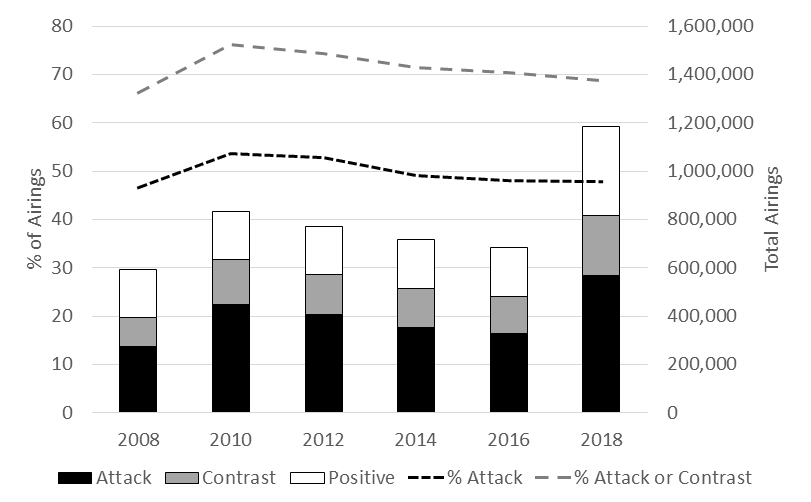
\includegraphics[width=\textwidth]{figures/negativa2}
	\caption{Volume e proporzione della negatività nelle elezioni federali americane tra il 2008 e il 2018. Kantar Media-CMAG, con analisi di Wesleyan Media Project.}
	\label{fig:negativa2}
\end{figure}

In controtendenza è invece uno studio del 2014 di Walter \citep{walter2014} in cui si compara la negatività registrata nelle campagne elettorali negli Stati Uniti dallo studio sopracitato di Geer con quella di 23 elezioni parlamentari di Germania, UK, e Olanda, avvenute tra il 1980 e il 2006. Da questo articolo risulta che la negatività media non sarebbe aumentata nelle campagne europee prese in considerazione [Fig. \ref{fig:negativab}]. I livelli medi registrati sono quindi i seguenti: 43\% per l'UK (il più alto), il 29\% per l'Olanda e il 18\% per la Germania. La media nello studi di Geer riguardo l'USA era invece del 36\%.  L’interpretazione dello studio quindi verte principalmente sui diversi sistemi elettorali degli stati anglofoni rispetto agli altri due stati europei: il bipolarismo tipico di questi paesi accentuerebbe l'utilizzo di campagna negativa, cosa che invece non succederebbe in Germania e Olanda, paesi con un arco parlamentare tradizionalmente più frammentato. Come vedremo nei prossimi capitoli, anche dal nostro studio emerge una dimensione del fenomeno in linea con quella rilevata da Walter per i paesi non anglofoni e non basati sul bipolarismo.
\begin{figure}
	\centering
	\begin{minipage}{.5\textwidth}
		\centering
		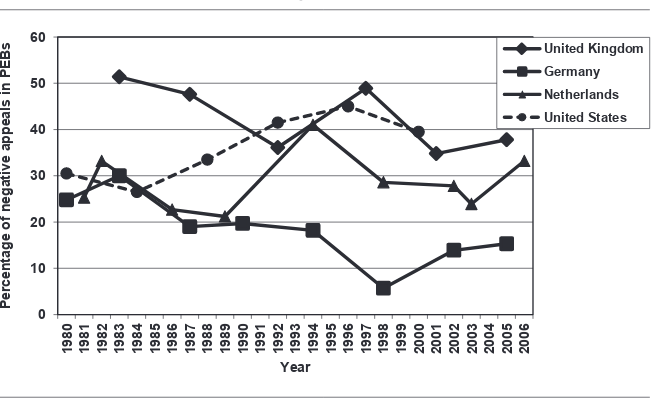
\includegraphics[width=0.99\linewidth]{figures/negativa22}
		\captionof{figure}{Quantità di campagna negativa durante le elezioni parlamentari dal 1980 al 2016, sono analizzati gli spot ufficiali dei partiti in televisione. Immagine pubblicata nello studio di Walter (2013).}
		\label{fig:negativab}
	\end{minipage}%
	\begin{minipage}{.5\textwidth}
		\centering
		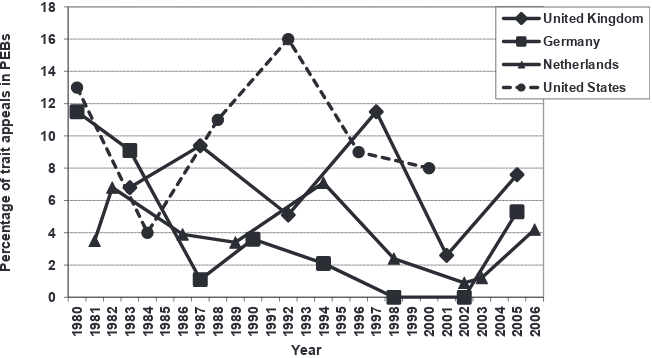
\includegraphics[width=1\linewidth]{figures/trait}
		\captionof{figure}{Quantità di campagna negativa rivolta a singoli candidati rivali nelle elezioni parlamentari dal 1980 al 2016. Immagine pubblicata nello studio di Walter (2013).}
		\label{fig:trait}
	\end{minipage}
\end{figure}

Altrettanto interessante per le analisi che verranno affrontate in questo elaborato, in particolare riguardo il target degli attacchi, un secondo grafico [Fig. \ref{fig:trait}] sempre della stessa ricerca di Walter\citep{walter2014}. Qui vengono illustrate le percentuali degli attacchi rivolti a un singolo candidato, arrivando sempre alla conclusione che il processo di \textit{personalization}, quanto meno negli attacchi, non ha subito significativi incrementi negli ultimi anni.

Anche in un altro studio \citep{papp2018} si afferma che la frammentazione dello scenario politico sia in grado di determinare il livello di negatività utilizzato dei politici in gara. Viene specificato come però, l'aumento non sia costante e lineare, ma avvenga secondo una curva a "U", in cui livelli alti di frammentazione, presupponendo la necessità di creare alleanze, riporti a una situazione simile a quella del bipolarismo, cioè a frammentazione   minima. Questo studio  ha analizzato gli articoli di prima pagina e il 5\% di tutti gli articoli relativi alle elezioni presenti nei principali quotidiani di nove paesi europei, nel mese precedente alle elezioni, dal 2005 al 2014. Non viene utilizzata direttamente la definizione direzionale di campagna negativa, ma viene effettuata una \textit{content analysis} in base al tono dei politici in riferimento ad avversari tramite una scala nominale che comprende toni negativi, positivi o neutri. Anche in questo caso non viene riscontrato un aumento nel corso degli anni presi in considerazione, ma solo variazioni tra un'elezione e l'altra o tra diversi paesi (danesi e tedesche le campagne meno negative, mentre Ungheria Inghilterra e Olanda si collocano all'estremo opposto). La media generale di negatività riscontrata si attesta al 46.8\%, 33.8\% quella positiva e il 19.4\% quella neutra. In uno dei grafici di questo studio [Fig. \ref{fig:negativau}] possiamo vedere la relazione tra frammentazione e tono negativo. Benchè non sia direttamente paragonabile con la presente ricerca, risulta interessante vedere come a una frammentazione intorno agli otto partiti in competizione (come nel caso delle elezioni italiane del 2019), la negatività si attesta intorno al 63\%.
\begin{figure}
	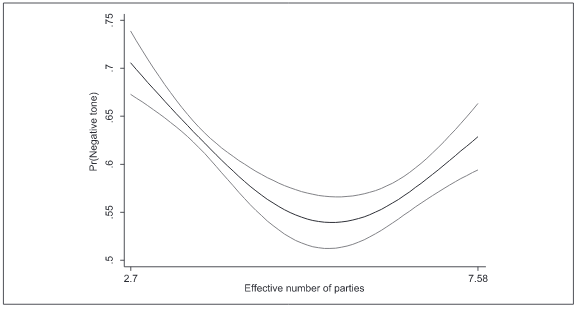
\includegraphics[width=\textwidth]{figures/negativau}
	\caption{Relazione tra il tono delle campagne politiche e il livello di frammentazione dell'arco politico. Immagine pubblicata nello studio di Papp (2018).}
	\label{fig:negativau}
\end{figure}
%Anche, altri ricercatori [Buell and Sigelman, 2009; Lau and Pomper, 2004] hanno criticato questi risultati

\subsection{In Italia}
Per quanto riguarda il panorama italiano è interessante lo studio di Ceron \citep{ceron2016}, in cui vengono categorizzati a mano sulla base della definizione direzionale di \textit{negative campaign} più di 15 mila tweet di politici in occasione delle elezioni nazionali del 2013. Qui le percentuali di campagna negativa rivolta a un avversario risultano decisamente inferiori a quelle d'oltre-oceano, attestandosi in media al 16.8\%. Vengono riscontrati risultati molto più elevati nei partiti non in carica in quel momento, come anche riscontrato nel nostro studio e in generale nella letteratura. Questo punto verrà trattato in modo più approfondito in un paragrafo successivo.

Un'altra ricerca che indaga proprio le elezioni europee del 2019 in Italia è quella di Seddone \citep{seddone2019}. Viene analizzata la negatività presente in questa campagna elettorale prendendo in considerazione i media tradizionali (cinque giornali e cinque televisioni) e la loro tendenza a utilizzare un tono negativo soprattutto nelle discussioni sull' Europa. Dai risultati si evince che i giornali sono più propensi, rispetto alle televisioni, a dare risalto a messaggi negativi: in media il 39.5\% dei messaggi sui giornali è stato codificato come negativo, rispetto al 32.5\% delle TV. In particolare però, Tg5 e Il Giornale, entrambi di proprietà di Silvio Berlusconi, hanno fatto registrare i valori più alti in assoluto (rispettivamente 47.5\% e 56.8\%), lasciando ipotizzare che l'elettorato di centrodestra, uscito con risultati inferiori alle aspettative nelle elezioni del 2018, sia stato particolarmente stimolato ad andare al voto tramite attacchi agli schieramenti sia più a destra che a quelli più a sinistra. Risulta interessante inoltre che i toni più negativi siano stati riscontrati su tematiche di politica interna piuttosto che verso l'Europa. Quest'ultimo tema risulta però differentemente coperto da giornali e TV: sugli schermi le tematiche europee appaiono con toni decisamente più negativi.

\section{Bias di negatività}
Trasversale a tutte le affermazioni e posizioni sostenute negli studi sul \textit{negative campaign}, risulta la teoria del \textit{negative bias}: l’effetto negatività fa in modo che i messaggi negativi risultino più persuasivi rispetto a messaggi positivi. Questo effetto è dimostrato anche in uno studio sull’attenzione, in cui vengono fatti eseguire dei “color-naming task”, per indagare le valutazioni automatiche \citep{pratto1991}. In tutti e tre gli esperimenti condotti in questo studio, gli stimoli negativi ricevono in media l’85\% in più di attenzione e l’effetto viene riscontrato in tutti i partecipanti. E’ possibile rintracciare  le cause originarie di questo comportamento in una prospettiva evoluzionistica:, gli stimoli negativi vengono sovraesposti per difenderci dai pericoli di tutti i giorni.

Rozin e Royzman \citep{rozin2001}, nella loro rassegna, evidenziano come ci siano diversi effetti collegati a questo fenomeno e che non sia possibile ridurli a una teoria onnicomprensiva. Spinte a livello adattativo, evolutivo e meccanicistico contribuiscono a creare il \textit{negativity bias}.
In generale possiamo dire che “Bad is stronger than good” \citep{baumeister2001}. Le emozioni negative, come i feedback negativi, hanno maggiore impatto rispetto ai corrispettivi positivi poiché le informazioni a riguardo vengono elaborate in modo più approfondito.

Per quello che ci interessa in questo studio, è un risultato consolidato che gli elettori prestino maggiore attenzione ai messaggi negativi rispetto ai positivi e che la percezione di paura generata dalla negatività stimoli l’interesse nelle campagne politiche e riesca a mobilitare gli elettori più radicali.

%\section{I processi intergruppo}

\section{Cosa spinge a usare questo linguaggio nel contesto politico?}
I motivi che spingono a utilizzare questo tipo di linguaggio, in particolare nel contesto politico, possono essere raggruppati in tre filoni principali: l'efficacia riscontrate da messaggi negativi su media tradizionali e, più recentemente sui social media; la maggiore efficacia nel mobilitare l'elettorato da parte di questo tipo di campagna; i fattori contestuali al tipo di sistema elettorale e la generale polarizzazione del dibattito. Nei prossimi sottoparagrafi affronteremo queste tre linee di spiegazione in modo separato, nonostante siano fattori che procedono sempre di pari passo.

Un autore che indaga tutte queste possibili cause è Geer \citep{geer2012}. Nel suo articolo  discute tre ipotesi: la prima è che questo tipo di campagna risulti più efficace nel creare consenso attorno a un* candidat*. Questa spiegazione non risulta pienamente dimostrata ed è tuttora molto dibattuta, tuttavia l'autore cita questa convinzione comune che, anche se non sempre supportata da dati oggettivi, risulta trainare le strategie comunicative di molte campagne politiche.

La seconda indicazione emersa dallo studio è una forte correlazione (r =.88) tra la polarizzazione del dibattito e il livello di negatività espresso durante la campagna. A questo riguardo viene specificato che, anche in base a studi precedenti dello stesso autore \citep{geer2006}, risulta più probabile che sia la crescente polarizzazione a causare l'aumento della negatività e non il contrario, come afferma invece Ansolabehere in uno studio precedente \citep{anso1995}. Emerge, quindi, che la negatività generale di una campagna politica può derivare dal contesto elettorale. In seguito vedremo anche la relazione con un'altro aspetto del contesto politico: la frammentazione degli schieramenti.

La terza ipotesi riguarda i media tradizionali e la loro tendenza a sovraesporre questo tipo di contenuto poiché risulterebbe più coinvolgente per gli/le utenti. Un celebre esempio a riguardo è la campagne elettorale del 2004 in cui la  Swift Boat Veterans for Truth, un' associazione di veterani americani, ha diffuso un video (\thefootnote{\url{youtube.com/watch?v=V4Zk9YmED48}}) in cui si attaccava direttamente il candidato alla presidenza John Kerry, riportando diverse testimonianze in cui venivano smentite alcune sue dichiarazioni riguardo le azioni eroiche svolte durante la leva militare in Vietnam. La cosa interessante di questo episodio è che lo spot pubblicitario è stato trasmesso solo sulle televisioni di Iowa, Wisconsin e Ohio, raggiungendo circa un milione di elettori. A causa però della grande diffusione che ne è stata fatta da altri media, alla fine della campagna elettorale quasi l'80\% dell'elettorato dichiarava di conoscere l'episodio.
Un aspetto che non viene trattato in questo studio è invece la funzione svolta dai social media che verrà invece affrontata in questa rassegna.

\subsection{Negatività e medium}
La relazione tra il tono della campagna e i media viene discussa in vari articoli, in particolare vengono indagate l'esposizione di questi messaggi nei media tradizionali, e la maggiore predisposizione dei contenuti negativi a diventare virali sui social media.

\subsubsection{I media tradizionali}
Da almeno trent'anni a questa parte le istituzioni subiscono un processo di continua evolu-zione, dettata anche dal progressivo aumento della loro dipendenza dai mass media. Ancora prima dell'avvento dei social media, Mezzoleni e Schulz si interrogano su questo processo di \textit{mediatisation} della politica \citep{mazzoleni1999} e su come potrebbe diventare un cambiamento positivo o negativo per le democrazie di tutto il mondo. Dopo aver analizzato i trend nella fiducia nelle istituzioni, comparando diversi paesi, e dopo aver descritto come la professionalizzazione dei \textit{campaign strategist} sia ormai (nel '99) un fatto consolidato e in qualche modo collegato a un aumento della negatività del discorso politico, non arrivano a una conclusione univoca. Propongono, quindi, due teorie opposte. Da una parte le istituzioni starebbero andando verso una “media-driven democracy”, dall'altra sarebbe semplicemente in atto una “third age” della comunicazione politica, senza eccessive cattive ripercussioni sulla democrazia in sé. Viene però negata l'esistenza di prove a favore della nascita di un “party of the media”, il fatto cioè che le democrazie sarebbero in balia di partiti fondati da chi detiene il potere mediatico, sostenendo piuttosto che il consenso sarebbe sempre più organizzato attraverso i media e che quindi risulta fondamentale utilizzarli al meglio per vincere le elezioni, ma questo è possibile anche per chi non detiene il controllo dei media stessi. In quegli anni la vittoria di Fernando Collor de  Mello in Brasile, di Tony  Blair in Inghilterra e dello stesso Berlusconi in Italia, aveva infatti posto molti interrogativi sull'uso che questi politici avevano fatto di televisioni private e di strategie comunicative spregiudicate.

Come viene sottolineato in un articolo relativo alle elezioni olandesi del 2010 \citep{walter2010}, il medium sul quale viene diffuso un messaggio è molto rilevante per poterne analizzare il livello di negatività. Non tutti i canali di diffusione di informazioni sono ugualmente predisposti ad accogliere questo tipo di messaggi. Nello studio di Walter, prendendo in considerazione le comunicazioni degli stessi partiti, i dibattiti elettorali andati in onda sulle televisioni pubbliche e quelle commerciali e i principali quotidiani, vengono codificati tutti gli attacchi positivi e negativi con i rispettivi target. Dalle analisi effettuate risulta che le differenze tra i tre canali di comunicazione nell’esposizione delle campagne negative sono significative, dimostrandosi più elevate nei dibattiti televisivi rispetto a giornali e canali dei politici stessi [Fig. \ref{fig:negativa3a}]. Per quanto riguarda il target utilizzato, l’analisi evidenzia come più ci si allontana dal controllo diretto dei candidati sui messaggi, più questi riportano poco gli attacchi alle argomentazioni degli avversari (“issue”) per spostarsi su attacchi verso il candidato avversario (“value” e “trait”) [Fig. \ref{fig:negativa3b}].
\begin{figure}
	\centering
	\begin{minipage}{.5\textwidth}
		\centering
		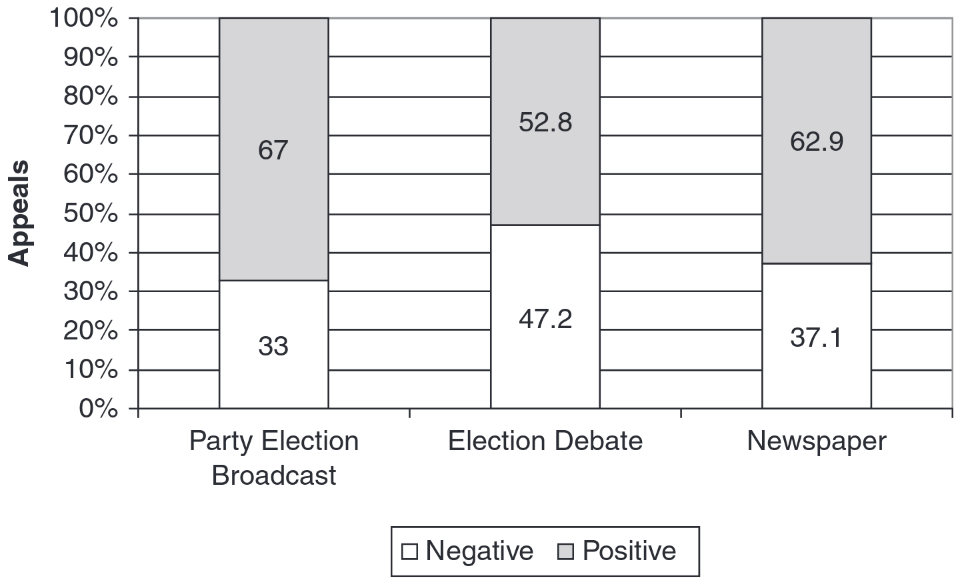
\includegraphics[width=\linewidth]{figures/negativa3b}
		\captionof{figure}{Quantità di campagna negativa registrata durante le elezioni olandesi del 2010, sono analizzati gli interventi dei partiti in tre diversi canali di comunicazione. Immagine pubblicata nello studio di Walter (2010).}
		\label{fig:negativa3a}
	\end{minipage}%
	\begin{minipage}{.5\textwidth}
		\centering
		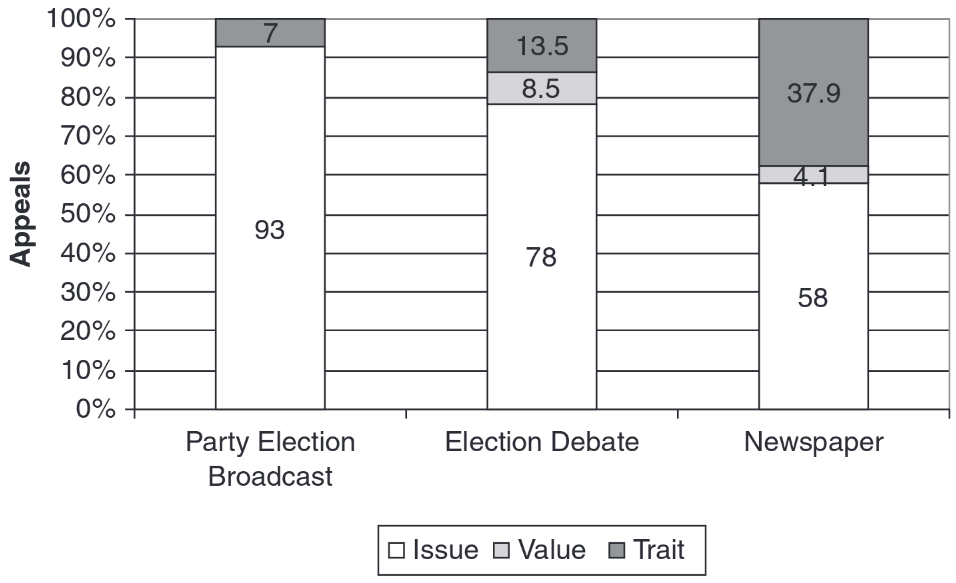
\includegraphics[width=\linewidth]{figures/negativa3a}
		\captionof{figure}{Tipo di target di campagna negativa registrata durante le elezioni olandesi del 2010, sono analizzati gli interventi dei partiti in tre diversi canali di comunicazione. Immagine pubblicata nello studio di Walter (2010)}
		\label{fig:negativa3b}
	\end{minipage}
\end{figure}

%ARTICOLO PACCO --> Ridout and Franz (2008).  They  demonstrate  a high correlation between levels of negativity in campaign ads and newspaper cover-age in several U.S. Senate races

In uno studio del 2008 in Scandinavia \citep{hansen2008}, viene riscontrato un fattore che potrebbe portare i politici ad aumentare sia la negatività delle loro campagne sia la sovraesposizione da parte dei media tradizionali di questo tipo di messaggio. Analizzando i principali quotidiani si riscontra un 22\% di articoli con citazioni diretta ad attacchi mossi da politici in corsa per le elezioni. Risulta dallo studio che però i politici abbiano solo un '8\% di questo tipo di attacchi nelle loro campagne, dimostrando con evidenza che i media tradizionali preferiscono parlare di questo tipo di critiche rispetto ad altre meno sensazionalistiche.

Anche uno studio sulle elezioni austriache del 2013 \citep{haselmayer2019} riporta risultati simili, dopo aver analizzato 1496 esternazioni dei partiti e 6512 notizie apparse sui giornali riguardo la campagna elettorale. Nella ricerca viene eseguita una codifica prima automatica e poi anche manuale atta a identificare quali delle esternazioni dei politici abbiano generato anche articoli sulla stampa. Ogni contenuto prodotto dai politici è stato anche codificato in base alla definizione direzionale di campagna negativa. I risultati rilevano come i messaggi negativi vengano maggiormente ripresi dalla stampa (17\% dei casi) se confrontati con quelli positivi (14\%). Viene, quindi, confermata l'ipotesi  secondo cui la negatività dei messaggi politici sarebbe un' efficace arma per accaparrarsi l'attenzione della stampa.

% https://iris.unito.it/retrieve/handle/2318/1730205/585493/105-Article%20Text-555-3-10-20191218%20%282%29.pdf

\subsubsection{Dai media tradizionali ai social network}
Se giornalisti e redattori di media tradizionali quali radio, stampa e TV devono sottostare a un codice deontologico necessario per entrare nell'albo di categoria che in qualche modo limita la possibilità di creare distorsioni nel riportare le affermazioni dei politici, il meccanismo di selezione dei contenuti mostrati agli/alle utenti dei social networks è gestito da un algoritmo proprietario che difficilmente può essere indicato come responsabile di distorsioni. Questi algoritmi sono stati definiti spesso come delle "black box" \citep{pasquale2015} dagli studiosi di \textit{algorithmic accountability} poichè, essendo alla base del valore commerciale delle piattaforme che li utilizzano, rimangono \textit{trade secrets} scarsamente accessibili agli utilizzatori e quindi anche agli studiosi. Alla base del concetto di \textit{black box} vi è  l'idea che a partire da un input, un sistema complesso ed opaco (\textit{black} appunto) restituisca un output visibile, facendo in modo che questo tipo di sistemi risultino, almeno in parte, oscuri non solo a chi ha accesso solo al risultato finale (un* utente che si ritrova uno specifico post in bacheca), ma anche a chi conosce gli input utilizzati dall'algoritmo (i programmatori della piattaforma). Alcuni studiosi si stanno interrogando su come ripensare gli algoritmi dei social networks per renderli più comprensibili e in grado di rispondere direttamente alle necessità di chi li utilizza \citep{reviglio2020}, ma la discussione rimane al momento ancora aperta.

Le scelte editoriali dei media tradizionali vanno quindi ricondotte al loro scopo informativo, ai bias individuali dei giornalisti e alla volontà degli editori di aumentare gli acquisti da parte dei loro clienti (l'obiettivo è un comportamento conscio, come l'acquisto di un determinato giornale). Nel caso dei social networks, invece, la selezione dei contenuti va ricondotta ad algoritmi pensati per massimizzare il tempo trascorso sulla piattaforma dagli/delle utenti (\textit{engagement}, non informatività) per poter aumentare il numero di pubblicità che è possibile somministrare e quindi vendere. Questi software vengono implementati a partire dalle abitudini degli/delle utenti, in particolare basandosi sul tempo trascorso su ogni tipologia di contenuto (agendo cioè ad un livello pre-conscio, tramite ad esempio l'analisi dei millisecondi con cui si scorre un post sulla propria bacheca) \citep{han2017}. Nonostante i due tipi di media abbiano modelli di \textit{business} diversi e valutino la riuscita della selezione di un contenuto in base a metodi diversi di stima del gradimento, dagli studi emerge, però, che in entrambi i casi i messaggi negativi sono preferiti.

\subsubsection{I social media}
Risultati simili a quelli rilevati sui media tradizionali sono infatti riscontrati in  analisi svolte sui social network.

Ad esempio, in un articolo relativo alle elezioni ungheresi del 2014 \citep{bene2017}, emerge come anche su Facebook la negatività abbia ripercussioni sulla viralità dei post condivisi dai politici. Analizzando 7048 post di 183 diversi candidati e dopo aver categorizzato ogni contenuto in base alla sua struttura (quantità di testo, immagine, tipo di immagine postata..) viene codificato manualmente il tono del messaggio, basandosi sulla presenza di "critiche, attacchi o espressioni di vergogna". Il risultato è molto interessante: solo il tono negativo dei messaggi è in grado di aumentare il numero di interazioni (likes, condivisioni e commenti). Come affermano gli autori, i contenuti negativi sono in grado di portare gli/le utenti ad esprimere le loro opinioni sul social in modo più consistente. A differenza dei media tradizionali, il social rende molto più rilevanti le reazioni degli elettori alle campagne politiche, poichè proprio sulla capacità di generare interazioni determina la visibilità dei contenuti stessi. In questo modo i commenti e i \textit{likes} (sia pro che contro il politico che li riceve) diventano direttamente parte della strategia comunicativa dei partiti, che non possono più prescindere da questi elementi se vogliono diffondere al meglio i propri contenuti.

In generale diversi studi \citep{berger2010} \citep{stieglitz2013} hanno trovato evidenze riguardo la diffusione e propagazione di messaggi basati sull'emotività, che risultano essere molto efficaci nei contesti dei social media. Analizzando 165mila tweet di comunicazione politica, Stieglitz e Dang-Xuan evidenziano come i tweet con forte emotività vengano condivisi molto più spesso rispetto a quelli neutrali e anche in modo più veloce, senza però riscontrare particolari differenze tra contenuti positivi e negativi. Hansen e colleghi \citep{hansen2011}, sempre su Twitter, trovano evidenze di una maggiore viralità dei contenuti negativi, ma con un campione diverso rispetto allo studio precedente, composto da notizie di attualità. Questa potrebbe essere la differenza in grado di spiegare i due diversi risultati.

Compiendo una \textit{sentiment analysis} di più di 100mila tweet contenenti messaggi rivolti a partiti o personaggi politici, uno studio svolto durante le elezioni tedesche del 2009 \citep{tumasjan2011} dimostra come Twitter sia un specchio fedele della realtà politica offline. Viene infatti mostrata una correlazione molto forte tra il numero di menzioni dei vari partiti ed i risultati delle elezioni. Questo conferma come, da almeno un decennio, i social networks siano parte integrante della vita politica e non si possano vedere solo come luoghi virtuali senza ripercussioni sulla vita reale. Attraverso l'utilizzo del software LIWC, gli autori analizzano anche il \textit{sentiment} dei contenuti analizzati, giungendo alla conclusione che sulla piattaforma può essere riscontrato, con buona approssimazione, il sentimento degli elettori in tempo reale.
%STUDIO CON LIWC CHE POTREBBE TORNARE UTILE --> Yu et al. (2008) who find that positive emotions outweigh negative emotions by more than 2 to 1 in an LIWC-based analysis of 18 years of congressional debates

Indagando nello specifico la piattaforma Twitter, Conover e colleghi \citep{conover2011} tramite clusterizzazione degli/delle utenti e network analysis di 355 milioni di tweet pubblicati durante le elezioni americane di \textit{midterm}, mostrano come i due tipi di interazioni (retweet e menzioni) possano produrre reazioni molto diverse [Fig. \ref{fig:twitternet}] e diversamente conflittuali. Chi usa il retweet prevalentemente discute con persone con cui è già d'accordo, le menzioni invece vengono utilizzate anche per discutere con persone lontane dal proprio punto di vista, aumentando la possibilità di scontri anche accesi.
\begin{figure}
	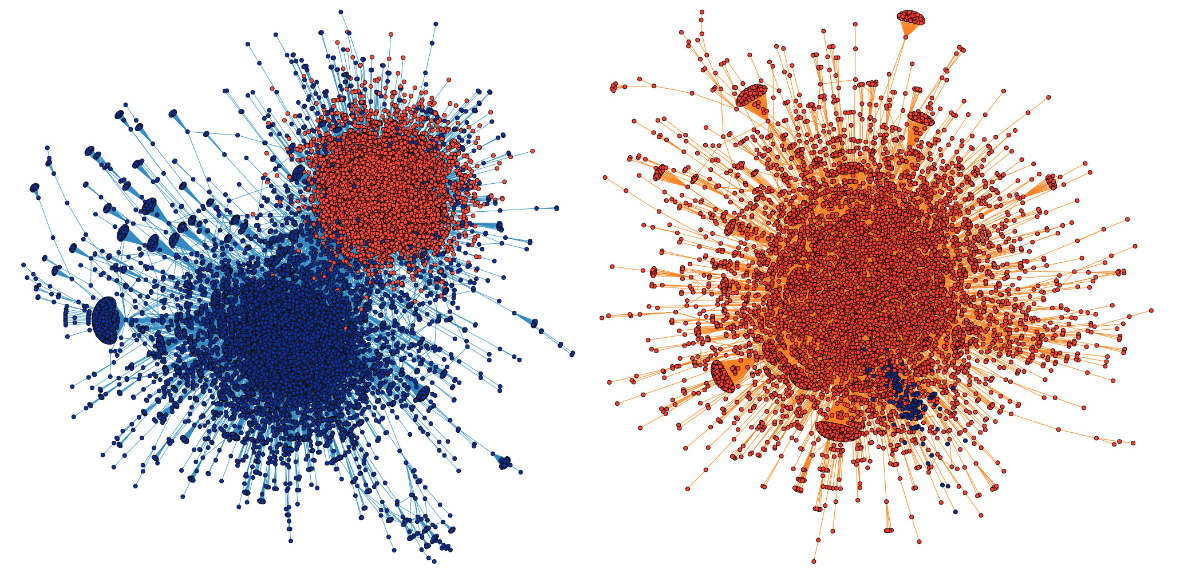
\includegraphics[width=\textwidth]{figures/twitternet}
	\caption{Network dei re-tweet (sinistra) e delle menzioni (destra) su twitter, i due colori rappresentano due cluster di utenti con opinioni politiche avverse. Mentre in un caso la struttura è molto più polarizzata, nel secondo network lo è meno. Immagine pubblicata nello studio di Conover e colleghi (2011).}
	\label{fig:twitternet}
\end{figure}


\subsection{Negatività e contesto elettorale}
Analizzando le elezioni danesi del 2005 Hansen e Pedersen \citep{hansen2008} confermano uno tra i principali punti fermi nella teoria del \textit{negative campaign}: i partiti d' opposizione sono i più propensi ad una campagna negativa. Spiegano questa relazione evidenziando come i partiti in carica abbiano molta più facilità ad ottenere attenzione dei media. Chi è invece all'opposizione ha bisogno di farsi notare tramite campagne negative in grado di sfruttare la sovraesposizione di questo tipo di messaggi nei media tradizionali.

Anche Druckman e Parkin \citep{druckman2010} mostrano evidenze a riguardo. Comparando 700 candidati al congresso statunitense nelle loro pubblicità in televisione e sui loro siti web durante tre diverse tornate elettorali consecutive (2002, 2004, 2006), dimostrano come la negatività sia praticamente uguale sui diversi media e come sia collegata invece a variabili quali la posizione istituzionale ricoperta al momento: chi è all'opposizione usa quasi 4 volte più campagne negative. Questo risultato, inoltre, viene avvalorato dal fatto che la negatività aumenta in base al livello di competizione per il posto in palio e i candidati arrivano a mostrare negatività ugualmente molto elevate quando il posto vacante è conteso da due politici entrambi non in carica.

Anche il già citato Walter \citep{walter2014}, nella sua comparazione delle campagne di diversi paesi europei, adducendo la tesi secondo cui le cause della negatività vadano riscontrate prevalentemente nel tipo di sistema elettorale, testa (e conferma) l'ipotesi della diversa propensione al \textit{negative campaign} tra politici in carica e non.

Un’altra tesi presente in letteratura è quella secondo cui sarebbero lo schieramento politico e relativa polarizzazione (destra o sinistra) a determinare i livelli di negatività. Curini e Martelli  \citep{curini2010}, hanno analizzato l’Italia dal dopoguerra alla fine della seconda repubblica (tra il 1946 e il 1994), in un periodo in cui era presente un bipolarismo chiamato “imperfetto” (tra Democrazia Cristiana e Partito Comunista). Considerando il tema della corruzione, mostrano come gli attacchi su questo argomento aumentino in modo inversamente proporzionale alla distanza ideologica che separa i partiti dalla controparte al governo.

\subsection{Negatività ed efficacia nelle campagne politiche}
Sebbene risulti abbastanza chiaro come le campagne negative siano più efficaci nella diffusione del messaggio, la letteratura non indica che questi attacchi siano sempre più efficaci dal punto di vista elettorale, come si evince dalla rassegna di Lau e colleghi \citep{lau2007}.

Sembra infatti che tali campagne siano in grado di mobilizzare elettori radicali in favore del soggetto che viene attaccato \citep{anso1995} ottenendo, così, risultati opposti a quelli desiderati. Inoltre, non sembra essere il modo migliore per contrapporre la propria immagine a quella di un rivale, a causa delle possibili ripercussioni negative nell'opinione dei propri elettori per l’uso di un linguaggio non consono a una figura istituzionale e alla discussione civile.

Ci sono, però, anche evidenze di segno opposto secondo le quali, in un sistema multipartitico, campagne negative rivolte ad avversari vicini alle proprie posizioni politiche portano gli indifferenti con posizioni simili a entrambi i partiti a supportare chi attacca rispetto a chi è attaccato \citep{curini2010}. È stato successivamente specificato  \citep{ceron2016} che però, l’effetto positivo su chi attacca viene accresciuto dall’essere allo stesso tempo sotto attacco: quando un partito è sotto attacco l’effetto “backlash” diminuisce poiché gli elettori difficilmente incolpano chi risponde ad altri attacchi per difendersi.

Uno studio condotto in Italia ha sondato gli effetti delle campagne negative sugli elettori a livello implicito ed esplicito \citep{carraro2010}. Dopo aver presentato affermazioni negative e positive verso avversari utilizzate da politici in corsa nelle ultime elezioni precedenti allo studio, sono state sottoposte ai partecipanti dell’esperimento valutazioni implicite ed esplicite dei candidati. I risultati mostrano come le valutazioni esplicite diminuiscano il gradimento dei candidati che attaccano ma non di quelli che subiscono gli attacchi, mentre a livello implicito il gradimento diminuisce per entrambi i candidati presentati.

Anche uno studio condotto sulle elezioni statunitensi \citep{fridkin2011} del 2006 giunge a conclusioni simili, prendendo in considerazione 30mila soggetti che hanno effettuato una valutazione dei candidati prima e dopo le elezioni e mettendoli in relazione con gli spot elettorali andati in onda in TV e la copertura mediatica che ne è stata fatta sui giornali. La particolarità di questo studio è che viene analizzato, oltre alla negatività dei messaggi, anche il livello di linguaggio incivile contenuto degli spot e la tematica più o meno rilevante per l’opinione pubblica. I risultati mostrano come linguaggi negativi e incivili influenzano effettivamente l’elettorato. In particolare messaggi su temi rilevanti con toni incivili abbassano le valutazioni per chi è in carica, mentre chi è all’opposizione non subisce questo effetto “backlash”.

Dall’altra parte, nello stesso studio \citep{fridkin2011}, viene anche sottolineato come gli attacchi negativi risultano però più presenti nella memoria degli elettori rispetto a quelli positivi. Risultato confermato in maniera diversa anche da un altro studio \citep{perloff1992}, in cui vengono confrontate le opinioni sulle campagne negative di consulenti e giornalisti politici, mostrando come entrambi pensino che possano avere importanti effetti sul comportamento dei votanti, indicando l’appello alle emozioni come una delle tecniche più utile per raggiungere gli elettori.

In generale, comunque, è importante considerare che gli attacchi negativi possono essere rivolti sia ad aspetti personali del candidato rivale che ai suoi valori e al suo programma. Nel secondo caso il “backfire” è molto minore che nel  primo caso \citep{carraro2010}.






%PARAGRAFO RIMOSSO
%\section{Questo tipo di campagna è legittima?}
%geer 2006 --> libro che spiega perché è giusto fare campagne negative

%Geer asks us to reject the starting assumption that attack ads are bad. In fact, he argues that democracy requires candidates to attack each other. His argument is simple but powerful: All advertisements, by their very nature, exaggerate the truth. But this point applies equally to negative and positive ads
%
%Lau, R. R. (2006). In Defense of Negativity: Attack Ads in Presidential Campaigns. Perspectives on Politics, 4(4), 772-773. --> fa riassunti di diversi libri.
%
%Nello stesso filone e negli stessi anni, ma con posizioni antitetiche, si pone Mayer. Il suo articolo "In Defense of Negative Campaigning." \cite{mayer1996}, cerca di mostrare come evidenziare i difetti altrui, con tutti gli attacchi necessari, sia utile per informare al meglio gli elettori sulle scelte da compiere. Facendo l'esempio di molti libri che analizzano le politiche attuali, partire dall'analisi dei difetti delle misure in atto è praticamente un \textit{must} retorico per poter illustrare le proprie proposte in grado di migliorare la situazione.













